\documentclass[11pt, oneside]{article} 
\usepackage{geometry}
\geometry{letterpaper} 
\usepackage{graphicx}
	
\usepackage{amssymb}
\usepackage{amsmath}
\usepackage{parskip}
\usepackage{color}
\usepackage{hyperref}

\graphicspath{{/Users/telliott_admin/Tex/png/}}
% \begin{center} 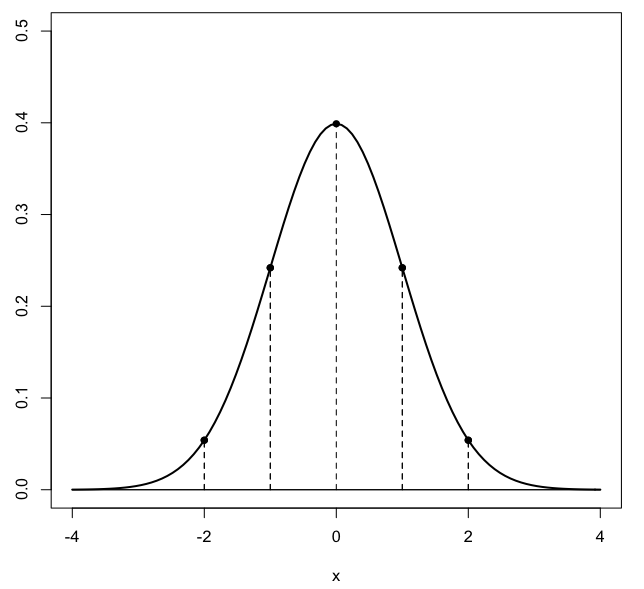
\includegraphics [scale=0.4] {gauss3.png} \end{center}

\title{Change of variables}
\date{}

\begin{document}
\maketitle
\Large

\label{sec:Change_of_variables}

We usually pick a coordinate system with the axes perpendicular, scaled in the same units, with the label $x$ for horizontal and $y$ for vertical.  But for some problems, it can be useful to change the coordinate system.  There are a number of possible ways to do this, as we'll see.  

There are also some basic rules to follow to insure that the areas and other integrals determined in the new coordinate system match up with those in the standard one.

Probably the simplest example is a linear stretching of one dimension, say, the $x$-axis.  Let's think about the problem of determining the area of the rectangle with one corner at $(0,0)$ and the other corner at $(2,1)$.  Although it seems like overkill, we're going to use single variable calculus to do it.  The upper edge is $y = f(x) = 1$.

\[ A = \int_{x=0}^{x=2} f(x)\ dx = \int_0^2 1\ dx = x  \ \bigg |_{0}^{2} = 2 \]

It's not strictly necessary to write the $1$ for $f(x)$ but I try to do it, to remind myself that we are looking for an area and haven't just forgotten some other $f(x)$.

The answer seems to be correct.

Now, define a new variable $u$ which is exchanged at a rate of 2 $u$'s for every $x$.  If 
\[ x = 1\Rightarrow u = 2 \]
\[ x = 0\Rightarrow u = 0 \]
This means that 
\[ u  = 2x \]
We leave $y$ unchanged.

We take the exact same shape, (with no change in the area), but change the horizontal coordinate system to be defined in terms of $u$.  The point $(2,1)$ becomes the point $(4,1)$ in the new coordinate system.  So we write
\[ A = \int_{u=0}^{u=4} f(u)\ du  \]
(This is wrong, but bear with me).  

We have adjusted the limits of integration, since before we had the upper limit of $x=2$, now we have the upper limit of $u=4$.  That part is correct.  $f(x)$ is a constant, so everywhere $f(x) = f(u) = 1$ no matter the value of $x$ (or $u$).

Our mistake is that $du \neq dx$.
\[ du = 2\ dx \]
\[ \frac{1}{2} du = dx \]
so we substitute
\[ A = \int_{x=0}^{x=2} f(x)\ dx =  \int_{u=0}^{u=4} f(u)\ \frac{1}{2}du \]
\[ =  \frac{1}{2} \int_0^4 f(u)\ du \]
\[ = \frac{1}{2} \int_0^4 1\ du \]
\[ =  \frac{1}{2} \times 4 = 2 \]
which is correct.

We can do the very same problem in an even more complicated way, using multi-variable calculus.  Above, we imagine that what we are doing is slicing the area vertically into many slices with tiny width $dx$ and height $f(x)$ and adding all these together.  

We can also imagine that we divide the area up into many little boxes of $dA$ and do the summation this way:
\[ A = \iint\limits_{R} 1 \ dA \]
The little boxes of area $dA$ have width $dx$ and height $dy$.
\[ A = \iint\limits_{R} 1 \ dA =   \int_{y=0}^{y=1} \int_{x=0}^{x=2} 1 \ dx \ dy  \]
We evaluate the \emph{inner} integral first, \emph{keeping $y$ constant}.
\[ \int_{x=0}^{x=2} 1 \ dx =  x  \ \bigg |_{0}^{2} = 2  \]
Then do the outer integral:
\[ = \int_{y=0}^{y=1}  2 \ dy  = 2y   \ \bigg |_{0}^{1} = 2  \]
(The real advantage of this is that we can substitute another function for $f(x,y) = 1$---see the Center of Mass chapter).  I introduce the two variable method as a way of approaching the next two problems.

\subsection*{Circle}
Consider a circle of radius $a$ centered at the origin.
\[ x^2 + y^2 = a^2 \]
\[ y = \sqrt{a^2-x^2} \]
This problem is symmetrical so we will only do it one way, integrating over $dy$ first.  
\begin{center} 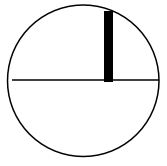
\includegraphics [scale=0.5] {dint7.png} \end{center}

Again, we will do the area function, and we will do only the first quadrant
\[ \int_{x=0}^{x=a}  \int_{y=0}^{y=\sqrt{a^2-x^2}} \ dy \ dx \]
The inner integral is just
\[ \int_{y=0}^{y=\sqrt{a^2-x^2}} \ dy = \sqrt{a^2-x^2} \] 
so now we have for the outer integral
\[ \int_{x=0}^{x=a}  \sqrt{a^2-x^2} \ dx \]

Substitute
\[ x = a \cos \theta \]
\[ dx = -a \sin \theta \ d \theta \]
For the limits we will have, when
\[ x = 0 \Rightarrow \theta = \pi/2 \]
\[ x=a \Rightarrow \theta= 0\]
 
Then
\[ \int_{x=0}^{x=a}  \sqrt{a^2-x^2} \ dx \]
\[ = -\int_{\theta=\pi/2}^{0} \sqrt{a^2-a^2 \cos^2\theta} \ a \sin \theta \ d \theta \]
\[ = \int_{0}^{\pi/2} \sqrt{a^2-a^2 \cos^2\theta} \ a \sin \theta \ d \theta \]
\[ =  a^2 \int_{0}^{\pi/2} \sin^2 \theta \ d \theta \]
\[ = \frac{a^2}{2} \ [ \theta - \sin \theta \cos \theta \ ] \ \bigg |_{0}^{\pi/2} \]
\[ = \frac{a^2}{2} \frac{\pi}{2} =  \frac{\pi}{4} a^2 \] 

\subsection*{Circle again}

Let's try to find the area of a circle of radius $a$ in a different way.  In terms of $x$ and $y$ we had previously
\[  \iint\limits_{R}  \ dA = \int_{x=0}^{x=a} \int_{y=0}^{y=\sqrt{a^2-x^2}} \ dy \ dx \]
\[ = \int_{x=0}^{x=a} \sqrt{a^2-x^2}  \ dx \]

There is an easier way to do this than trig substitution, and that is to change to polar coordinates.  A naive attempt is
\[  \iint\limits_{R}  \ dA = \int_{\theta=0}^{\theta=2 \pi} \int_{r=0}^{r=a} \ dr \ d \theta \]
\[ = \int_{\theta=0}^{\theta=2 \pi} a \ d \theta = 2 \pi a \]

Obviously, this is wrong.
What happened is that the area element for a little bit of area $dA$ has an extra factor of $r$:
\[ dA = dx \ dy = r \ dr \ d \theta \]
This is the area element dA in the $xy$-plane.  
\begin{center} 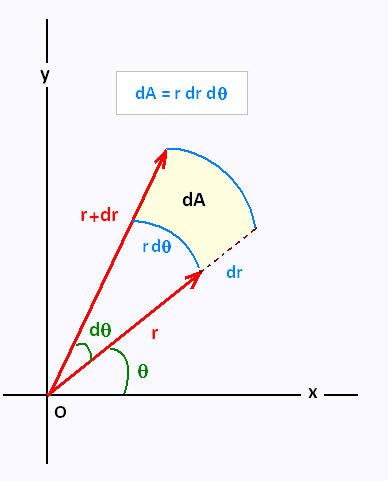
\includegraphics [scale=0.6] {polar_area_element.png} \end{center}
Notice that the little piece of the radius $dr$ is a length, but the little piece of angle $d \theta$ is \emph{not a length}.  To get the length of the curvy part of the area element $dA$, we need to multiply the change in angle by the radius.  So
\[ dA = r d \theta \cdot \ dr \]
(usually written $r \ dr \ d \theta$).  To get an area, you must multiply two lengths.

\url{http://www.scientificsentence.net/Equations/CalculusIII/}

The length of the curvy segment of arc depends on how far out we are on the radius.

Finishing the problem:
\[ \iint\limits_{R}  \ dA = \int_{\theta=0}^{\theta=2 \pi} \int_{r=0}^{r=a} \ r \ dr \ d \theta \]
\[ = \int_{\theta=0}^{\theta=2 \pi} \frac{1}{2}a^2 \ d \theta = \pi a^2 \]

\section*{sphere volume}

\subsection*{method:  multi-variable calculus}

Now, let's try to figure out what the volume elements are for a sphere.
\begin{center} 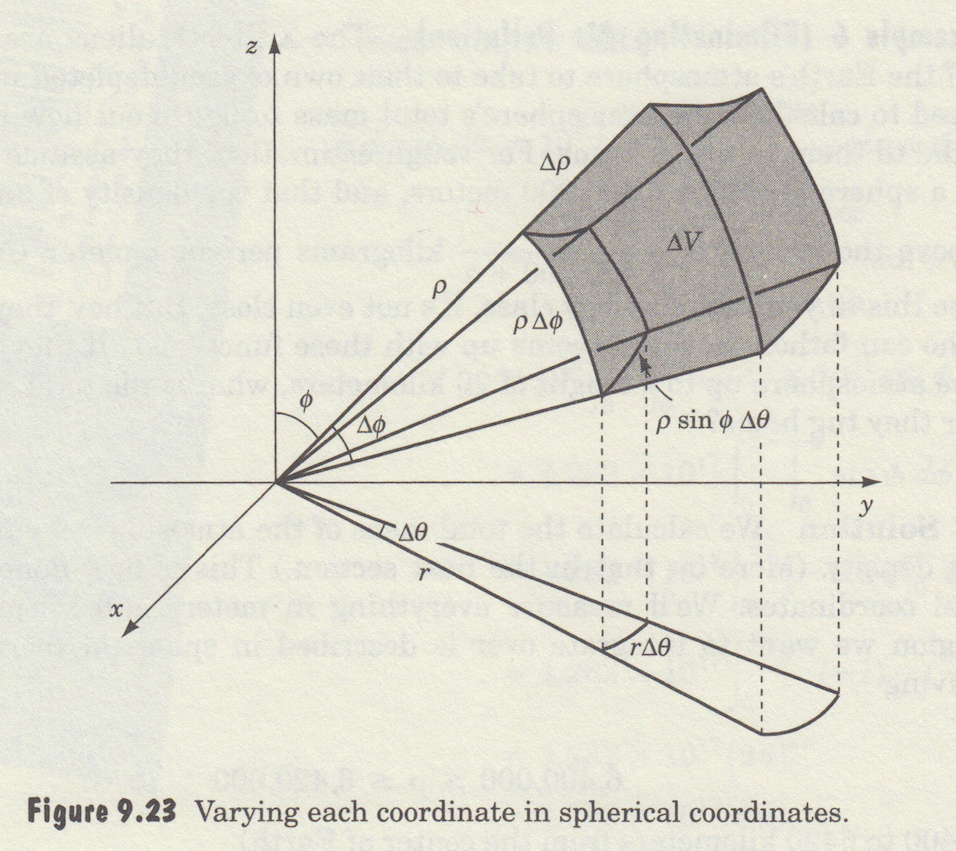
\includegraphics [scale=0.3] {sphcoord.png} \end{center}
The standard way of labeling everything (the parametrization) begins with the polar angle.  This is the angle made by the volume element with the positive $z$-axis.  

The mathematicians call this angle $\phi$.  (The physicists call it $\theta$, but don't get me started).

The other angle is the standard one from polar coordinates, which is the angle with the positive $x$-axis, or $\theta$.  And for the sphere, usually the radius is denoted by $\rho$ rather than $r$, just to remind us that we are dealing with a sphere.

The two straight sides of the otherwise curvy little box $dV$ lie along two radii, and their length is just $d \rho$.  

The two sides which are somewhat vertical here lie on two different great circles, centered on the origin.  Imagine traveling around the world on a constant line of longitude.  You would travel about $24,901$ miles, the circumference of the earth.

To get the length, multiply $d \phi$ by the radius $\rho$ to obtain $\rho \ d \phi$.  

The tricky parts of the volume elements are the sides involving $d \theta$.  These also lie on a circle, but it is not a great circle.  Instead these are horizontal slices perpendicular to the $z$-axis.  

Imagine traveling around the world on a constant line of latitude, say at $60$ degrees north.  You would not travel $24,901$ miles but something less than that.  The radius and circumference of this circle depend on $\phi$.

Looking at the projection in the $xy$-plane, you should see that the circle has radius $r$ where $r = \rho \sin \phi$ and therefore the length of these guys is
\[ r \ d \theta = \rho \sin \phi \ d \theta \]

Putting it all together we get two factors of $\rho$ and one of $\sin \phi$ so:
\[ dV = \rho^2 \sin \phi  \ d \theta \ d \phi \ d \rho \]
Obtaining the volume element is the hard part.

The triple integral can be done in any order.  Most commonly $\rho$ is done first and $\theta$ last, with the $\theta$ integral independent of the others by symmertry, so it contributes $2 \pi$ to the final result.
\[ dV = \rho^2 \sin \phi  \ d \rho \ d \phi \ d \theta \]

\subsection*{volume integral}

We set up a triple integral
\[ V = \iiint dV \]
\[ = \int_{\theta = 0}^{2 \pi} \int_{\phi = 0}^{\pi}  \int_0^{R} \rho^2 \sin \phi  \ d \rho \ d \phi \ d \theta \]
The integral is easy because the different parts are independent.  The only tricky part is the upper bound on $\phi$, which is equal to $\pi$.  Imagine rotating the circle in the $xy$-plane through the full range of $\pi$.  We need rotate only by a half-circle to cover the entire volume.

Using independence, we can even rewrite this as
\[ = \int_{\theta = 0}^{2 \pi} d \theta \int_{\phi = 0}^{\pi}  \sin \phi \ d \phi \int_0^{R} \rho^2  \ d \rho \]
We get a factor of $2 \pi$ from the outside integral and $R^3/3$ from the inside, and the middle is
\[ \int_{0}^{\pi}  \sin \phi \ d \phi = - \cos \phi \ \bigg |_{0}^{\pi} = 2\]
Altogether, that is
\[ 2 \pi \cdot \frac{\rho^3}{3} \cdot 2 = \frac{4}{3} \pi R^3 \]

\end{document}